\section{Experiments}\label{sec:expriments}
\todo{Skal jeg ikke nævne C-version, Python-version, compiler-version etc.? Det har jeg set i andre artikler.}

To test or hypotheses we have conducted several experiments on the different implementations of the Forward and the Backward algorithms. All the experiments have been conducted on a ThinkPad W540 with 32GB RAM and an Intel I7-4700MQ running 64bit Debian 10. All the experiments have 3 replicates in order to minimize random fluctuations due to other processes of the computer.
All experiments were conducted through the Python-library as described in \textbf{section \ref{sec:pb}}.

\subsection{BLAS vs Conventional}\label{sec:A1}
To test or\todo{our} initial hypothesis, that a linear algebra implementation utilizing BLAS for the Forward and Backward algorithm is faster than the conventional version, we conducted the following experiment.

The experiment was conducted with an varying input size starting with $100'000$ going up to $1'000'000$, increasing $100'000$ each time. The state space was varied as well: from $10$ to $400$. Varying the state space allows us to test the consistency of the performance over all the influencing variables. The experiment is show in \textbf{figure \ref{fig:A1}}. 

\textbf{Figure \ref{fig:A1}} clearly shows that the BLAS version is faster than the conventional implementation in all experiments. It is also clear that the efficiency ratio between the BLAS version and the conventional implementation increases with the size of the state space. This supports our initial hypothesis. 

\begin{figure}[H]
  \centering
  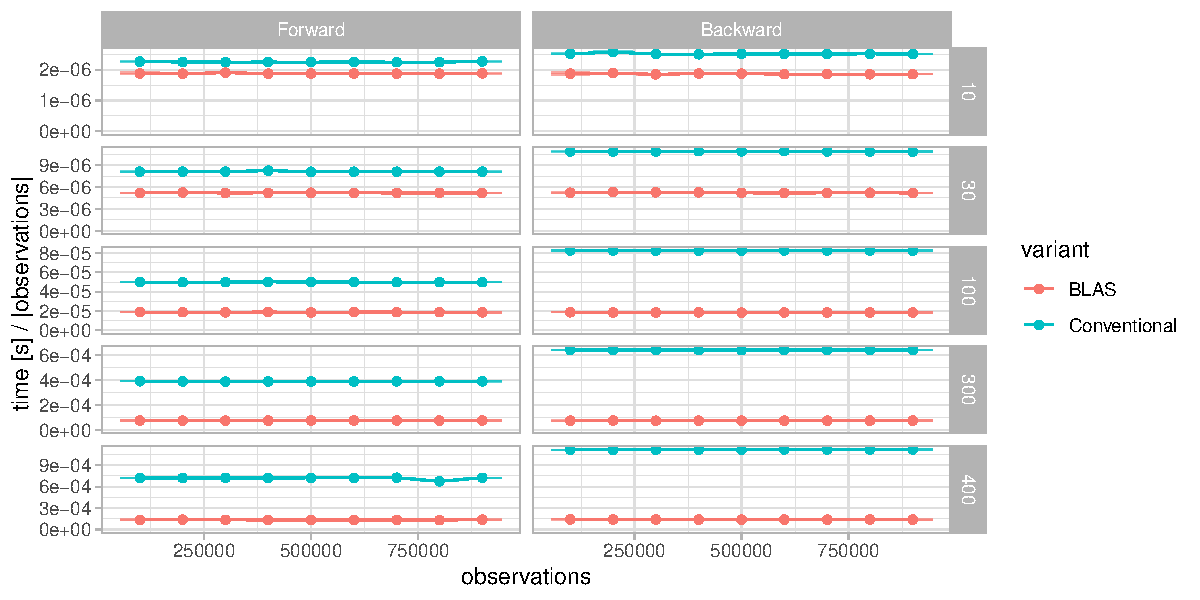
\includegraphics[scale=0.85]{figures/figure_A1.pdf}
  \caption{\small{Forward and Backward running time experiment for the linear algebra and the conventional implementations. The vertical axis shows time divided by number of observations. Error bars denote standard deviation of 3 replicates. Alphabet size: 4.}}
  \label{fig:A1}
\end{figure}

To verify that the algorithms scale with their theoretical running times the measured time is divided with the input size on \textbf{figure \ref{fig:A1}}. It is clear that the algorithms follow their theoretical running times for both implementations. 

\textbf{Figure \ref{fig:A1}} implies that the BLAS version is faster than the conventional implementation supporting our hypothesis. \todo{Especially when the statespace increases.}

\subsubsection{Baum-Welch and Posterior decoding}\label{sec:A2}

In the following experiment we want to test our hypothesis, that if we increase the speed of the Forward and the Backward algorithms we will see an equal speed up in the Baum-Welch and the Posterior decoding algorithms. \textbf{Figure \ref{fig:A2}} shows the experiment running the Baum-Welch and the Posterior decoding algorithms using the conventional and BLAS version of the Forward and Backward algorithms.

\begin{figure}[H]
  \centering
  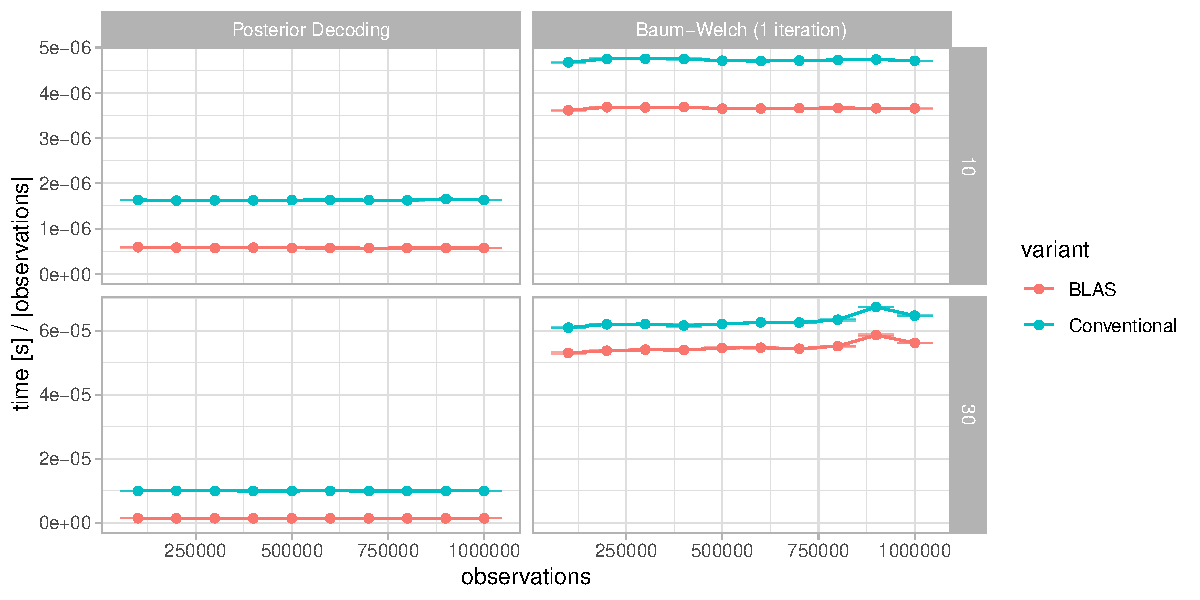
\includegraphics[scale=0.85]{figures/figure_A2.pdf}
  \caption{\small{Posterior decoding and Baum-Welch running time experiment with the BLAS version and the conventional implementation. The vertical axis shows time divided by number of observations. Error bars denote standard deviation of 3 replicates. Alphabet size: 4.}}
  \label{fig:A2}
\end{figure}

To verify that the algorithms scale with their theoretical running times, we have divided the measured time with the input size on \textbf{figure \ref{fig:A2}}. It is clear that the algorithms follow their theoretical running times for both algorithms.

\textbf{Figure \ref{fig:A2}} clearly shows that there is an equivalent increase in speed for both the Baum-Welch and Posterior decoding algorithms, supporting our hypothesis.

\subsection{Sparse instance of HMM}
\todo{titelforslag: Sparse HMM}

To test our hypothesis for the sparse instance of an HMM, we implemented versions of the Forward and the Backward algorithm utilizing the CSR format and the RSB format as described in \textbf{section \ref{sec:impel}}. In the following two experiments we tested the two implementations against each other, and in the last experiment we tested the fastest of these (RSB) against the BLAS implementation.

We define density as a value between 0 and 1, where a density of 0 signifies the most sparse valid transition matrix where only one value per row is non-zero. When the density goes towards 1, the density of the matrix is equivalent to the filling percentage of the matrix. \todo{forkert. 'filling percentage' antyder et proportionelt forhold. Skriv i stedet: 'When the density goes from 0 to 1, the number of edges in theta goes from n to n*n, where n is the number of hidden states. }

All the experiments are conducted with an input size of $100'000$ observables, whilst varying the density of the transition matrix and the state space. For all the experiments we use a dense emission matrix with $4$ observables. 

\subsubsection{RSB vs. CSR}

In the following experiment we want \todo{slet 'want to'} to compare the RSB and CSR implementations of the Forward and the Backward algorithms. The results of this experiment are shown on \textbf{figure \ref{fig:B3}}. 

\begin{figure}[H]
  \centering
  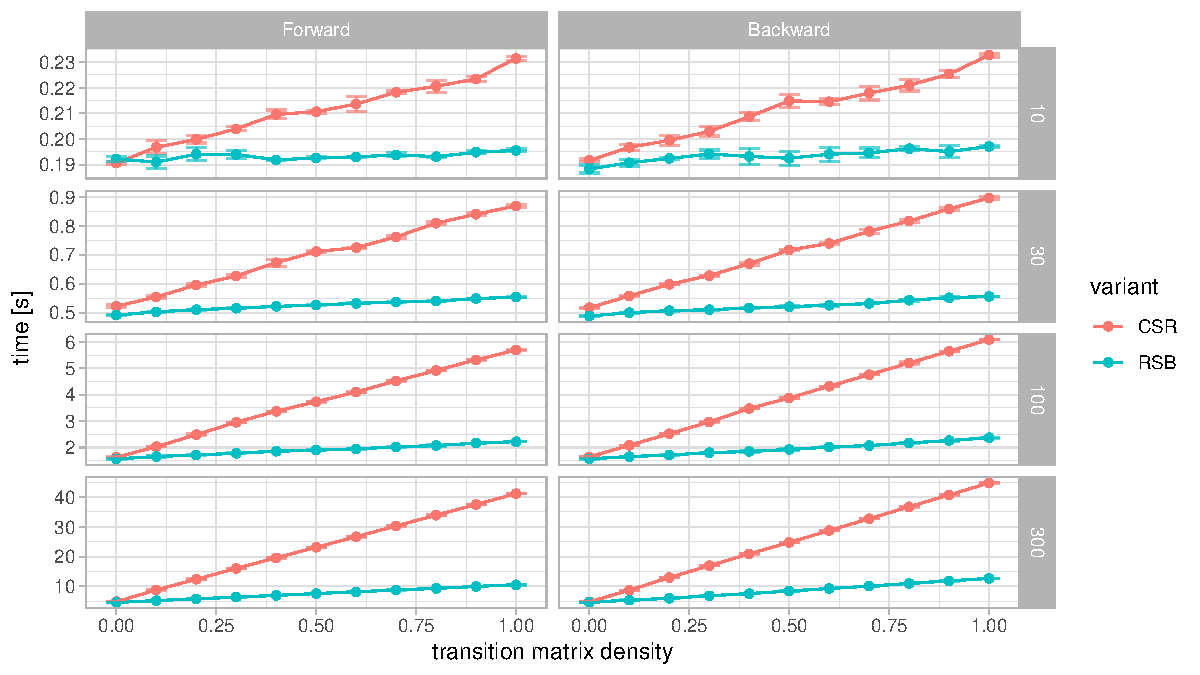
\includegraphics[scale=0.85]{figures/figure_B3.pdf}
  \caption{\small{Comparison of the two sparse implementations: CSR and RSB. Forward and Backward algorithms with a fixed input of size $100'000$ and varying state space and density. Alphabet size of 4.}}
  \label{fig:B3}
\end{figure}

From \textbf{figure \ref{fig:B3}} it is clear that the RSB implementation is faster than the CSR implementation for all combinations of state-space size and density.

\subsubsection{BLAS vs RSB}\label{sec:B1}

In the following experiment we want to test our hypothesis, that the implementations of the Forward and the Backward algorithms optimized for sparse instance of an HMM utilizing libRSB yields a speed up compared to our density-ignorant BLAS version when the transition matrix is sparse.

\begin{figure}[H]
  \centering
  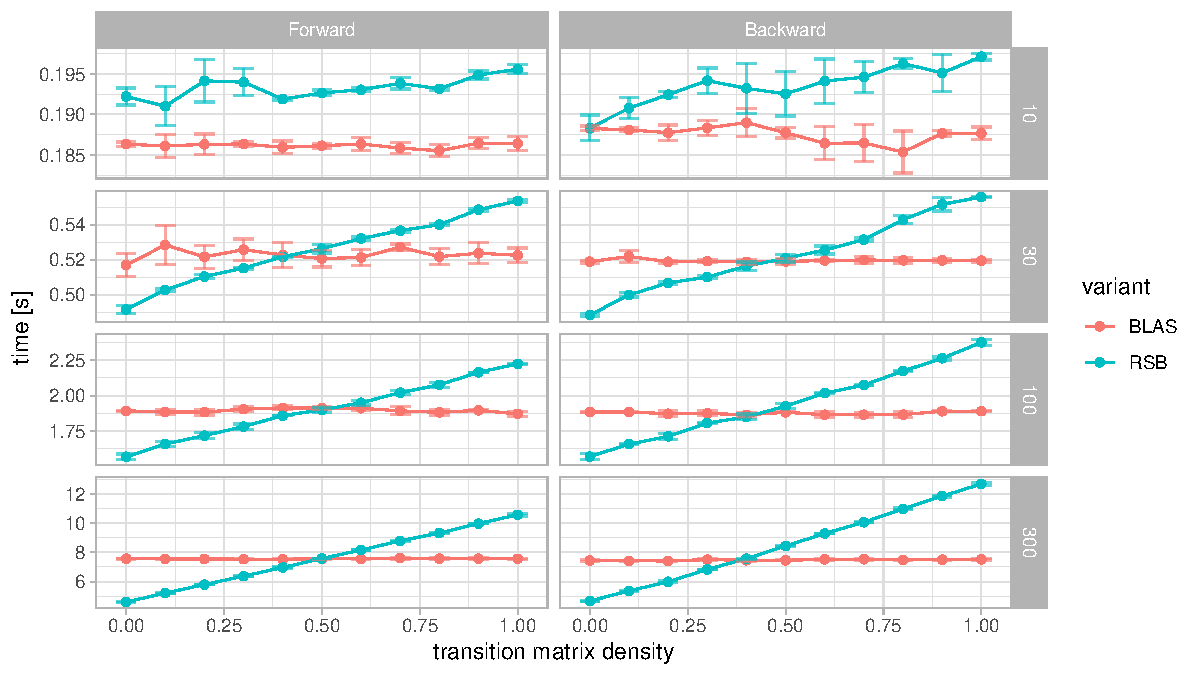
\includegraphics[scale=0.85]{figures/figure_B1.pdf}
  \caption{\small{Experiment of the BLAS and RSB implementations of the Forward and Backward algorithms with a fixed input of size $100'000$ and varying state space and density. Alphabet size of 4.}}
  \label{fig:B1}
\end{figure}

\textbf{Figure \ref{fig:B1}} shows that for the state spaces in the range of $30$ and up, the RSB implementation has a speed up relative to the BLAS version when the density is below $0.375$. This speed up goes for both the Forward and the Backward algorithms. It seems like the advantage of the Forward algorithm is stabilizing at a density of $0.5$ and for the Backward algorithm it is stabilizing at $0.375$.

This supports or hypothesis, that it is possible to achieve a speed up for the sparse instances of the HMM when utilizing the sparseness. 
The increase in speed should also be present in the Baum-Welch and Posterior decoding algorithms as implied in the results of \textbf{section \ref{sec:A2}}.

\subsection{Conclusion on experiments}
Throughout all of our experiments we have managed to support our hypotheses, that utilizing linear algebra increases the efficiency of the Forward and Backward algorithms in \textbf{section \ref{sec:A1}} and that this increase is present in the Baum-Welch and Posterior Decoding algorithms in \textbf{section \ref{sec:A2}}. We have also shown, experimentally, that utilizing the sparse implementation of matrix multiplications leads to a further increase in speed for sparse instances of the HMM in \textbf{section \ref{sec:B1}}.